\section*{\centering ANEXOS}

\vspace{0.3cm}

\phantomsection\label{anexo1}
\noindent \textbf{Anexo 1}

\vspace{0.2cm}

\begin{table}[H]
\footnotesize
\raggedright
\textbf{Tabla A.1} \\
\textit{Lista de Problemas Evaluados (Escala Likert)} \\[0.4em]

\centering
\begin{tabularx}{\linewidth}{c X >{\centering\arraybackslash}p{0.8cm} >{\centering\arraybackslash}p{0.8cm} >{\centering\arraybackslash}p{0.8cm} >{\centering\arraybackslash}p{0.8cm} >{\centering\arraybackslash}p{1.1cm}}
\hline
\textbf{N.°} & \textbf{Identificación del Problema} & \textbf{4\newline Ex.} & \textbf{3\newline Bu.} & \textbf{2\newline Reg.} & \textbf{1\newline Mal.} & \textbf{Total Puntaje} \\ 
\hline
1 & ¿Cómo calificas la búsqueda manual de datos de equipos en archivos Excel desactualizados? & 3 & 7 & 4 & 2 & 43 \\
\hline
2 & ¿Cómo calificas la recepción y comunicación por canales informales (WhatsApp/llamadas) sin registro? & 3 & 5 & 5 & 2 & 39 \\
\hline
3 & ¿Cómo calificas la descoordinación y reubicación de horarios por cruces en visitas \textit{in-situ}? & 2 & 5 & 7 & 2 & 39 \\
\hline
4 & ¿Cómo calificas el retraso en el escalamiento e identificación del historial de tickets previos? & 2 & 8 & 2 & 1 & 37 \\
\hline
5 & ¿Cómo calificas la verificación manual de términos y límites de servicio en contratos (SLA)? & 2 & 3 & 7 & 3 & 34 \\
\hline
6 & ¿Cómo calificas la elaboración manual de reportes e informes de rendimiento de fin de mes? & 1 & 3 & 6 & 4 & 29 \\
\hline
7 & ¿Cómo calificas la carencia de indicadores de rendimiento (KPIs) para evaluar el tiempo de respuesta del técnico? & 3 & 2 & 2 & 1 & 23 \\
\hline
\multicolumn{6}{r}{\textbf{Total General:}} & \textbf{244} \\
\hline
\end{tabularx} \\[0.4em]

\raggedright
{\small \textit{Nota.} Listado detallado de problemas evaluados mediante encuesta aplicada al personal de soporte técnico.}
\end{table}

\clearpage

\phantomsection\label{anexo2}
\noindent \textbf{Anexo 2}

\vspace{0.2cm}

\begin{table}[H]
\footnotesize
\raggedright
\textbf{Tabla A.2} \\
\textit{Tabla de Frecuencia y Distribución de Pareto} \\[0.4em]

\centering
\begin{tabularx}{\linewidth}{c X >{\centering\arraybackslash}p{1.4cm} >{\centering\arraybackslash}p{1.5cm} >{\centering\arraybackslash}p{1.6cm} >{\centering\arraybackslash}p{1.1cm}}
\hline
\textbf{N.°} & \textbf{Problemas / Causas Raíz} & \textbf{Puntaje} & \textbf{\% acumulado} & \textbf{Frecuencia acumulada} & \textbf{80 - 20} \\ 
\hline
1 & Búsqueda manual de datos de equipos en archivos Excel desactualizados & 43 & 17.62\% & 43 & 80\% \\
\hline
2 & Recepción y comunicación por canales informales (WhatsApp/llamadas) sin registro & 39 & 33.61\% & 82 & 80\% \\
\hline
3 & Descoordinación y reubicación de horarios por cruces en visitas \textit{in-situ} & 39 & 49.59\% & 121 & 80\% \\
\hline
4 & Retraso en el escalamiento e identificación del historial de tickets previos & 37 & 64.75\% & 158 & 80\% \\
\hline
5 & Verificación manual de términos y límites de servicio en contratos (SLA) & 34 & 78.69\% & 192 & 80\% \\
\hline
6 & Elaboración manual de reportes e informes de rendimiento de fin de mes & 29 & 90.57\% & 221 & 80\% \\
\hline
7 & Carencia de indicadores de rendimiento (KPIs) para evaluar el tiempo de respuesta del técnico & 23 & 100.00\% & 244 & 80\% \\
\hline
\multicolumn{2}{r}{\textbf{Total General:}} & \textbf{244} & \multicolumn{3}{c}{} \\ 
\hline
\end{tabularx} \\[0.4em]

\raggedright
{\small \textit{Nota.} Análisis acumulado de frecuencias y porcentajes bajo el principio de Pareto para los problemas del área de soporte técnico.}
\end{table}

\newpage

\phantomsection\label{anexo3}
\noindent \textbf{Anexo 3}

\vspace{0.2cm}

\begin{figure}[H]
\raggedright
\textbf{Figura A.1} \\
\textit{Diagrama de Pareto} \\[0.4em]
\caption{Diagrama de Pareto}
\label{fig:diagrama_pareto_anexo}

\centering
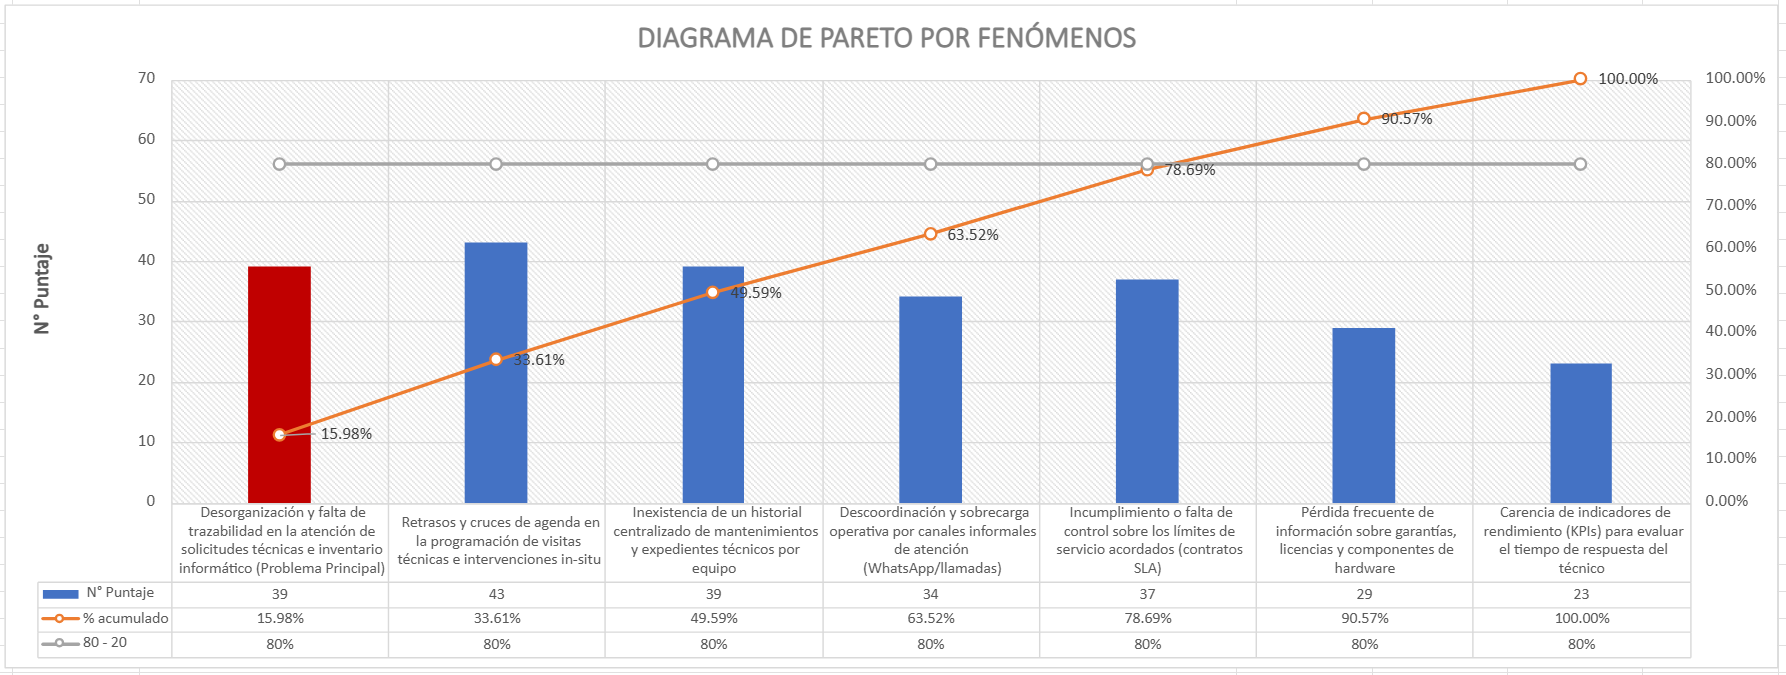
\includegraphics[width=1\linewidth]{img/diagrama_pareto.png} \\[0.2em]

\raggedright
{\small \textit{Nota.} Representación gráfica de la regla 80/20 que evidencia las causas principales a resolver en la gestión del HelpDesk.}
\end{figure}


\clearpage
\phantomsection\label{anexo4}
\hypertarget{anexo4_acta}{}

\noindent \textbf{Anexo 4}
\vspace{0.4em}

\begin{figure}[H]
    \centering
    \caption{Acta de Constitución del Proyecto (Parte 1)}
    \label{fig:acta_constitucion_1}
    \vspace{0.3em}
    \raggedright
    \textbf{Figura A.2} \\
    \textit{Acta de Constitución del Proyecto (Parte 1)} \\[0.3em]
    \centering
    % trim = [izquierda, abajo, derecha, arriba] en puntos (pt). Ajusta los valores si necesitas más o menos recorte.
    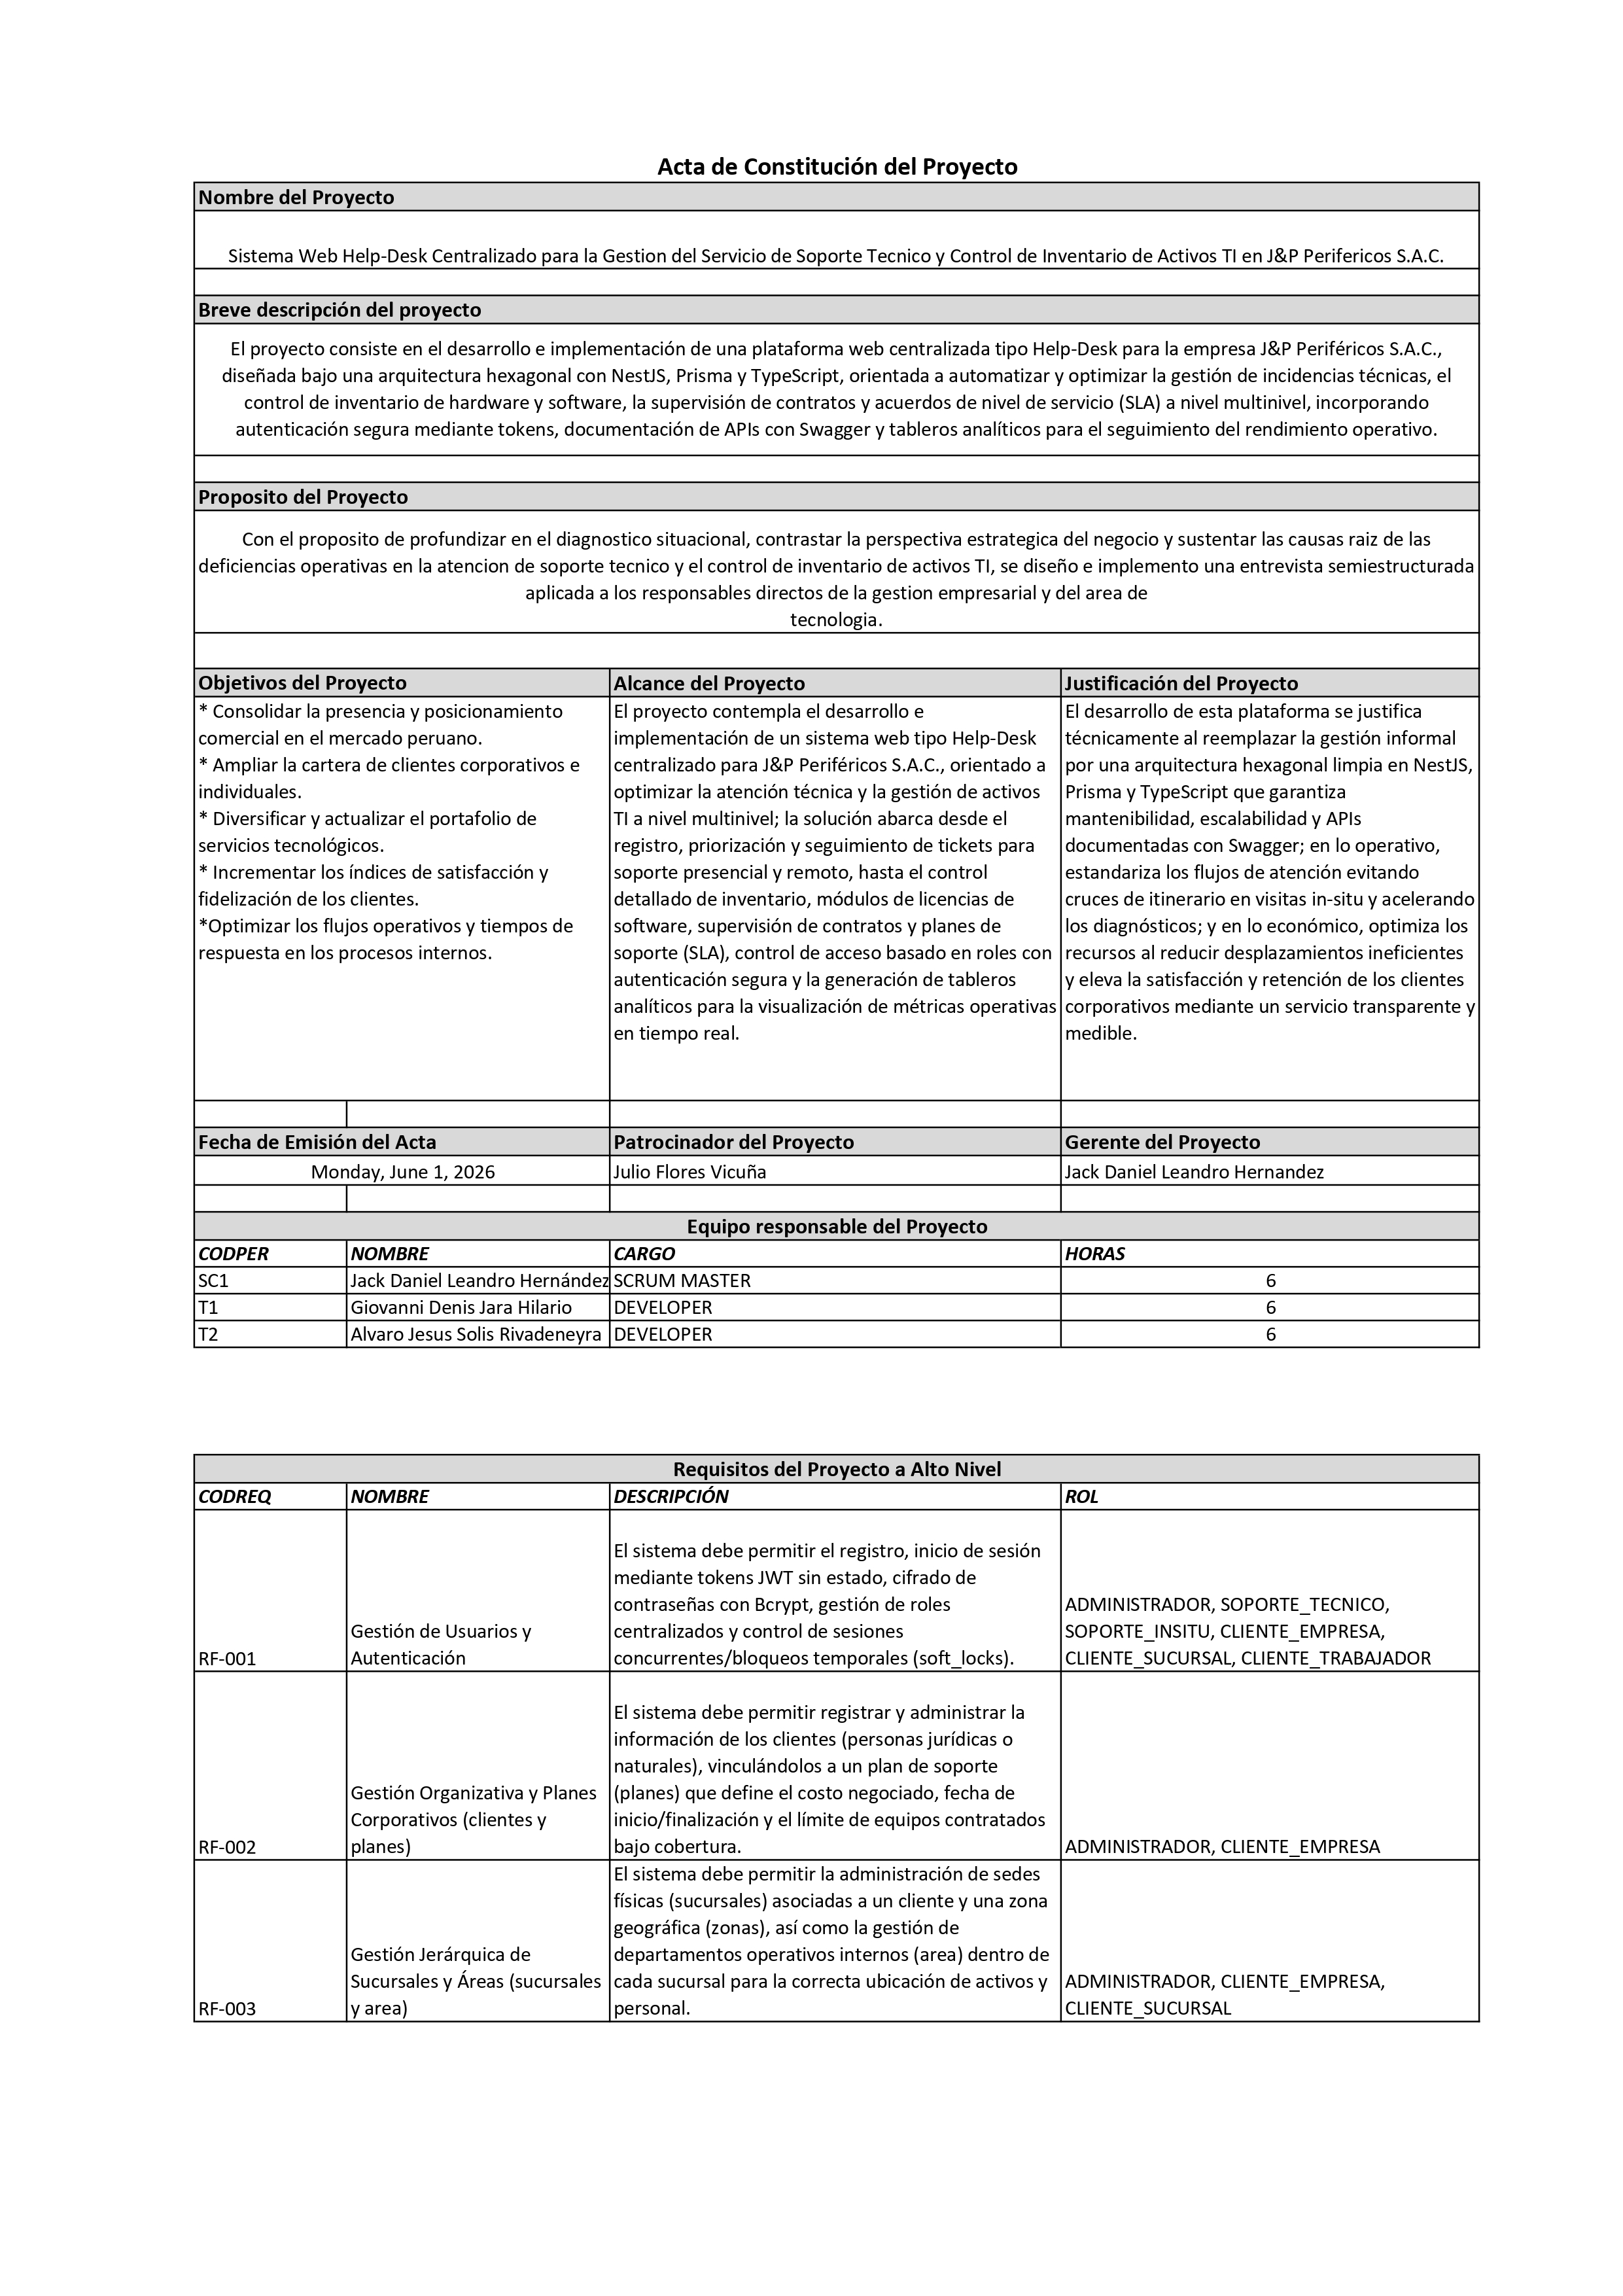
\includegraphics[width=0.82\linewidth, trim=0 80 0 40, clip]{img/Acta_Constitucion_HelpDesk_page_01} \\[0.3em]
    \raggedright
    {\small \textit{Nota.} Documento oficial de constitución, objetivos, alcance y equipo responsable de J\&P Periféricos S.A.C.}
\end{figure}

\clearpage

\begin{figure}[H]
    \centering
    \caption{Acta de Constitución del Proyecto (Parte 2)}
    \label{fig:acta_constitucion_2}
    \vspace{0.3em}
    \raggedright
    \textbf{Figura A.3} \\
    \textit{Acta de Constitución del Proyecto (Parte 2)} \\[0.3em]
    \centering
    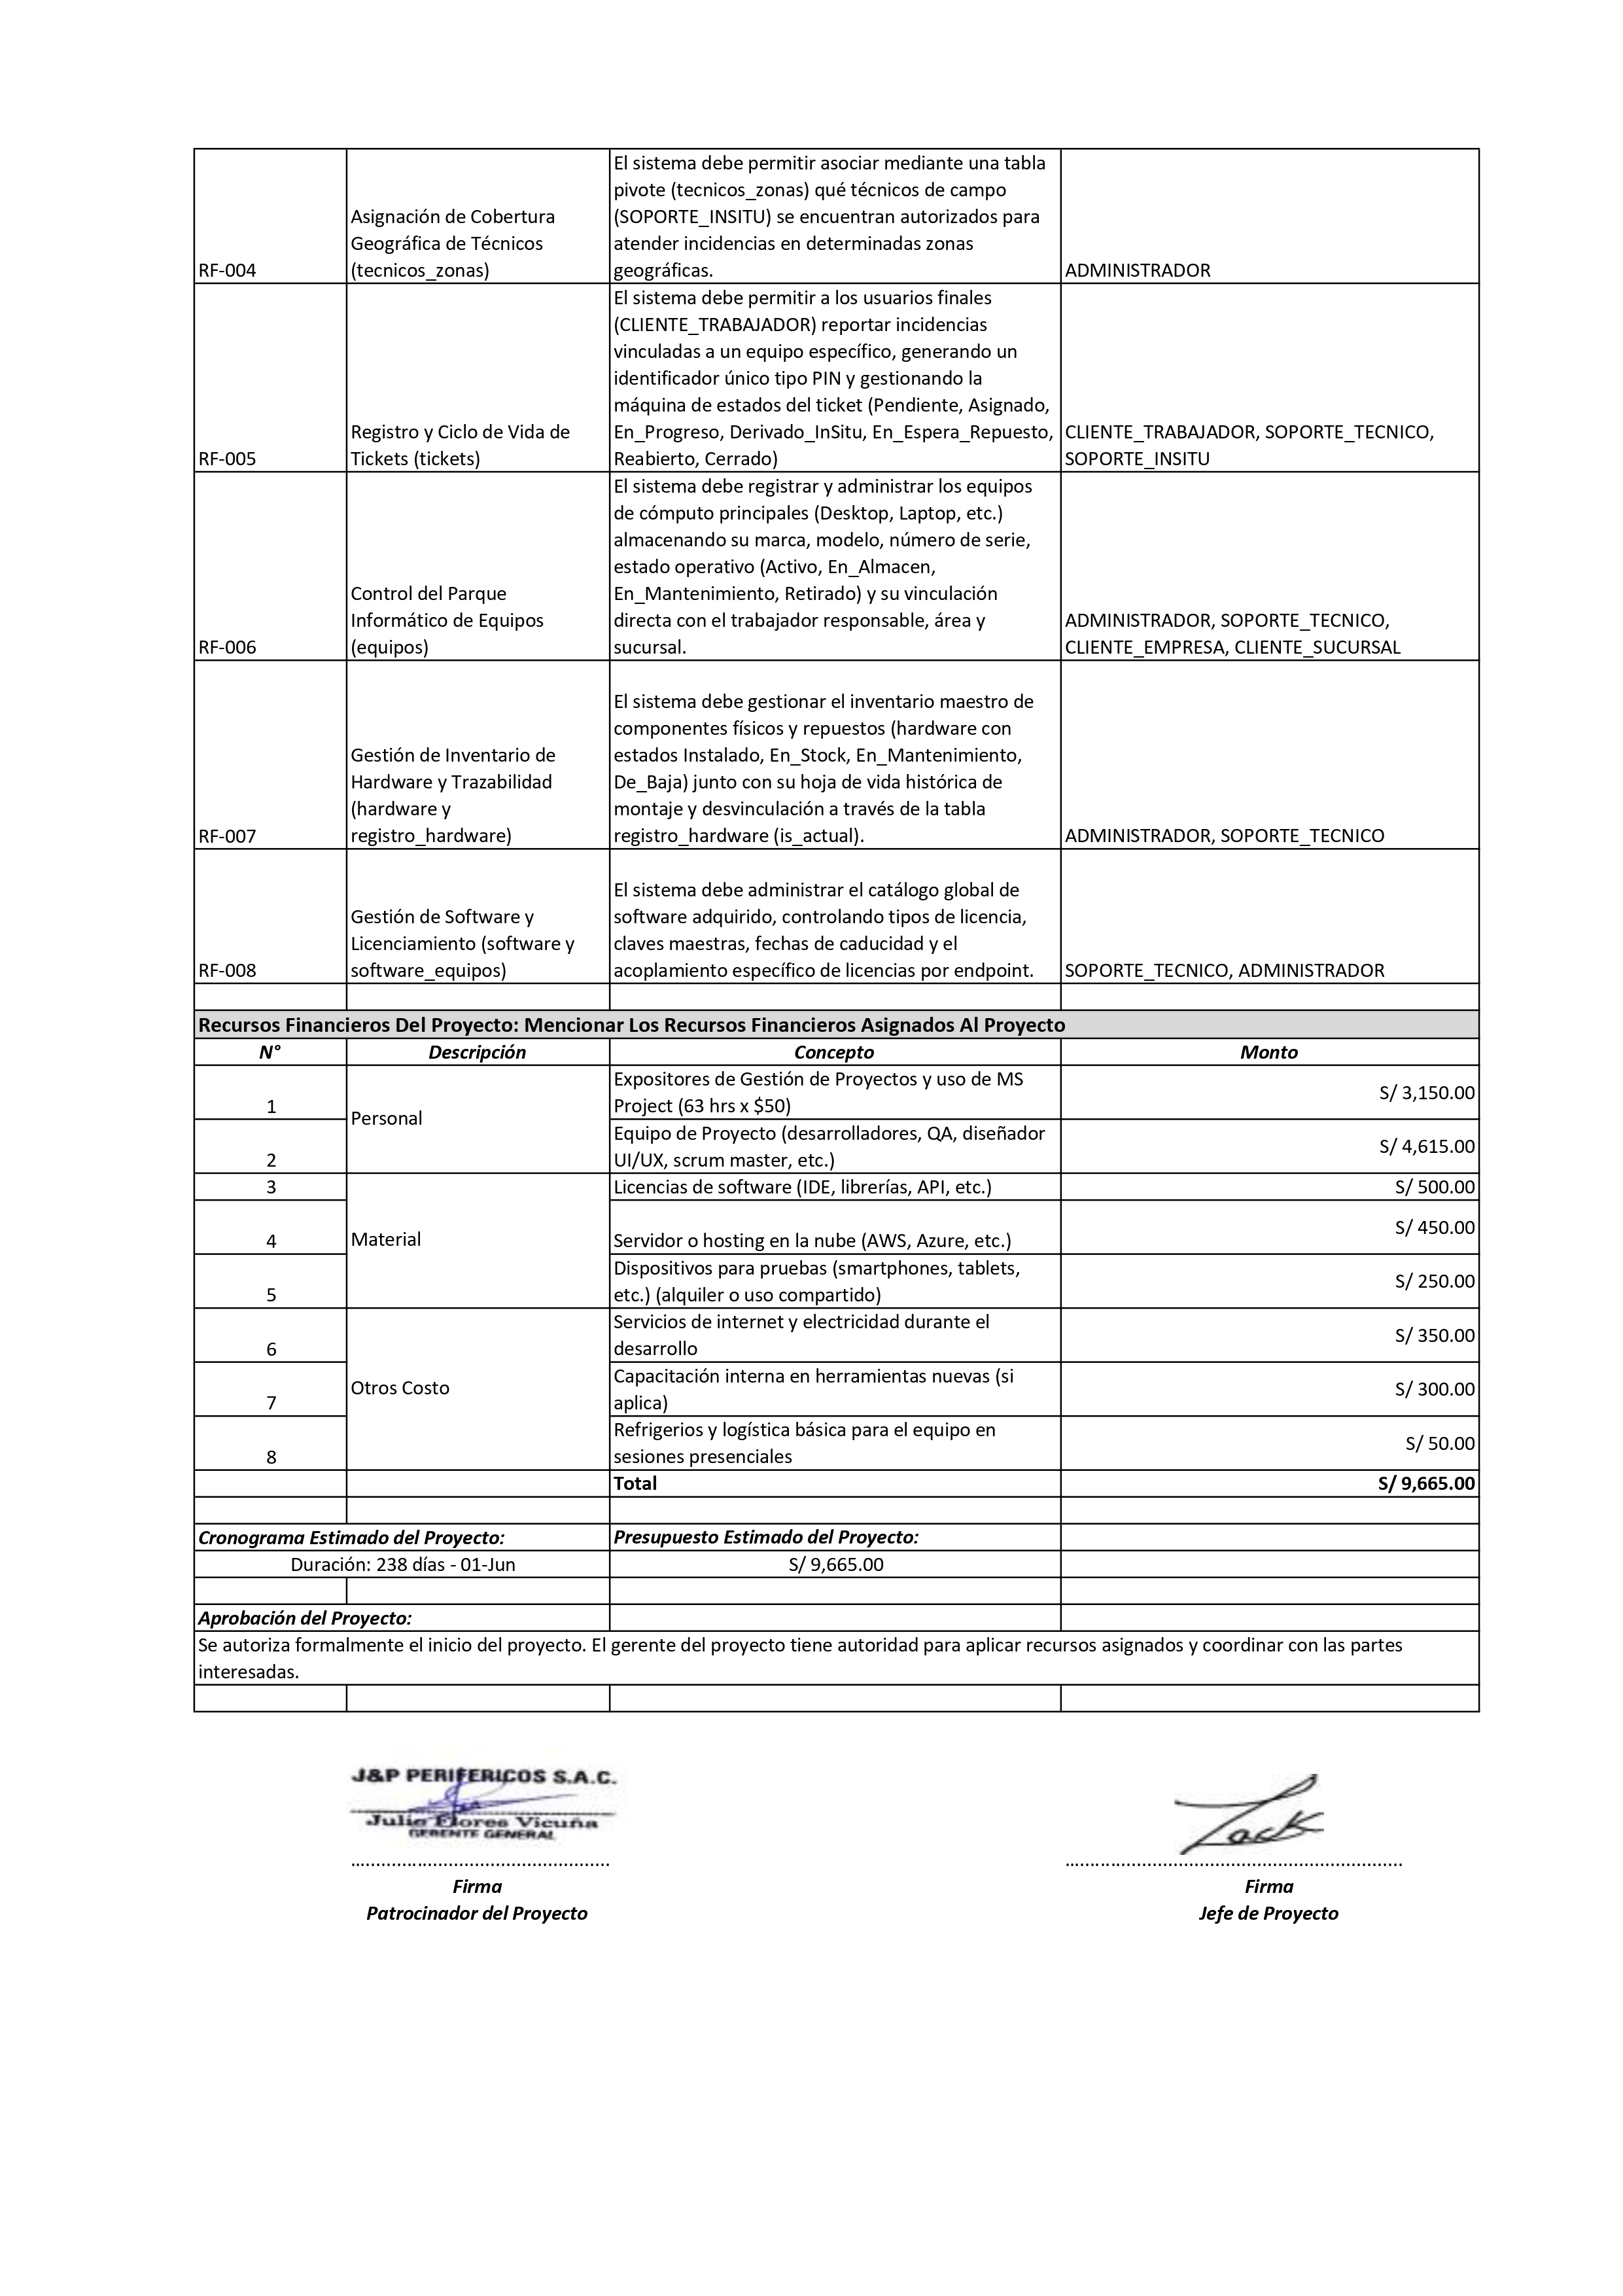
\includegraphics[width=0.82\linewidth, trim=0 120 0 40, clip]{img/Acta_Constitucion_HelpDesk_page_02} \\[0.3em]
    \raggedright
    {\small \textit{Nota.} Detalle de requerimientos a alto nivel, recursos financieros, cronograma y firmas de aprobación del proyecto.}
\end{figure}